\documentclass[a4paper,12pt]{article}

\usepackage[utf8]{inputenc}
\usepackage[french]{babel}
\usepackage[T1]{fontenc}
\usepackage{multirow,array}
\usepackage{graphicx}
\usepackage{a4wide}
\newcommand{\HRule}{\rule{\linewidth}{1mm}}

\begin{document}


%
%  TITLE
%

\begin{titlepage}

\begin{center}
\huge Easy porting of numerical simulation software to GPUs
\HRule \\
\medskip
{\Huge \bfseries The GMlib library} \\
\HRule
\end{center}

\begin{figure}[htbp]
\begin{center}
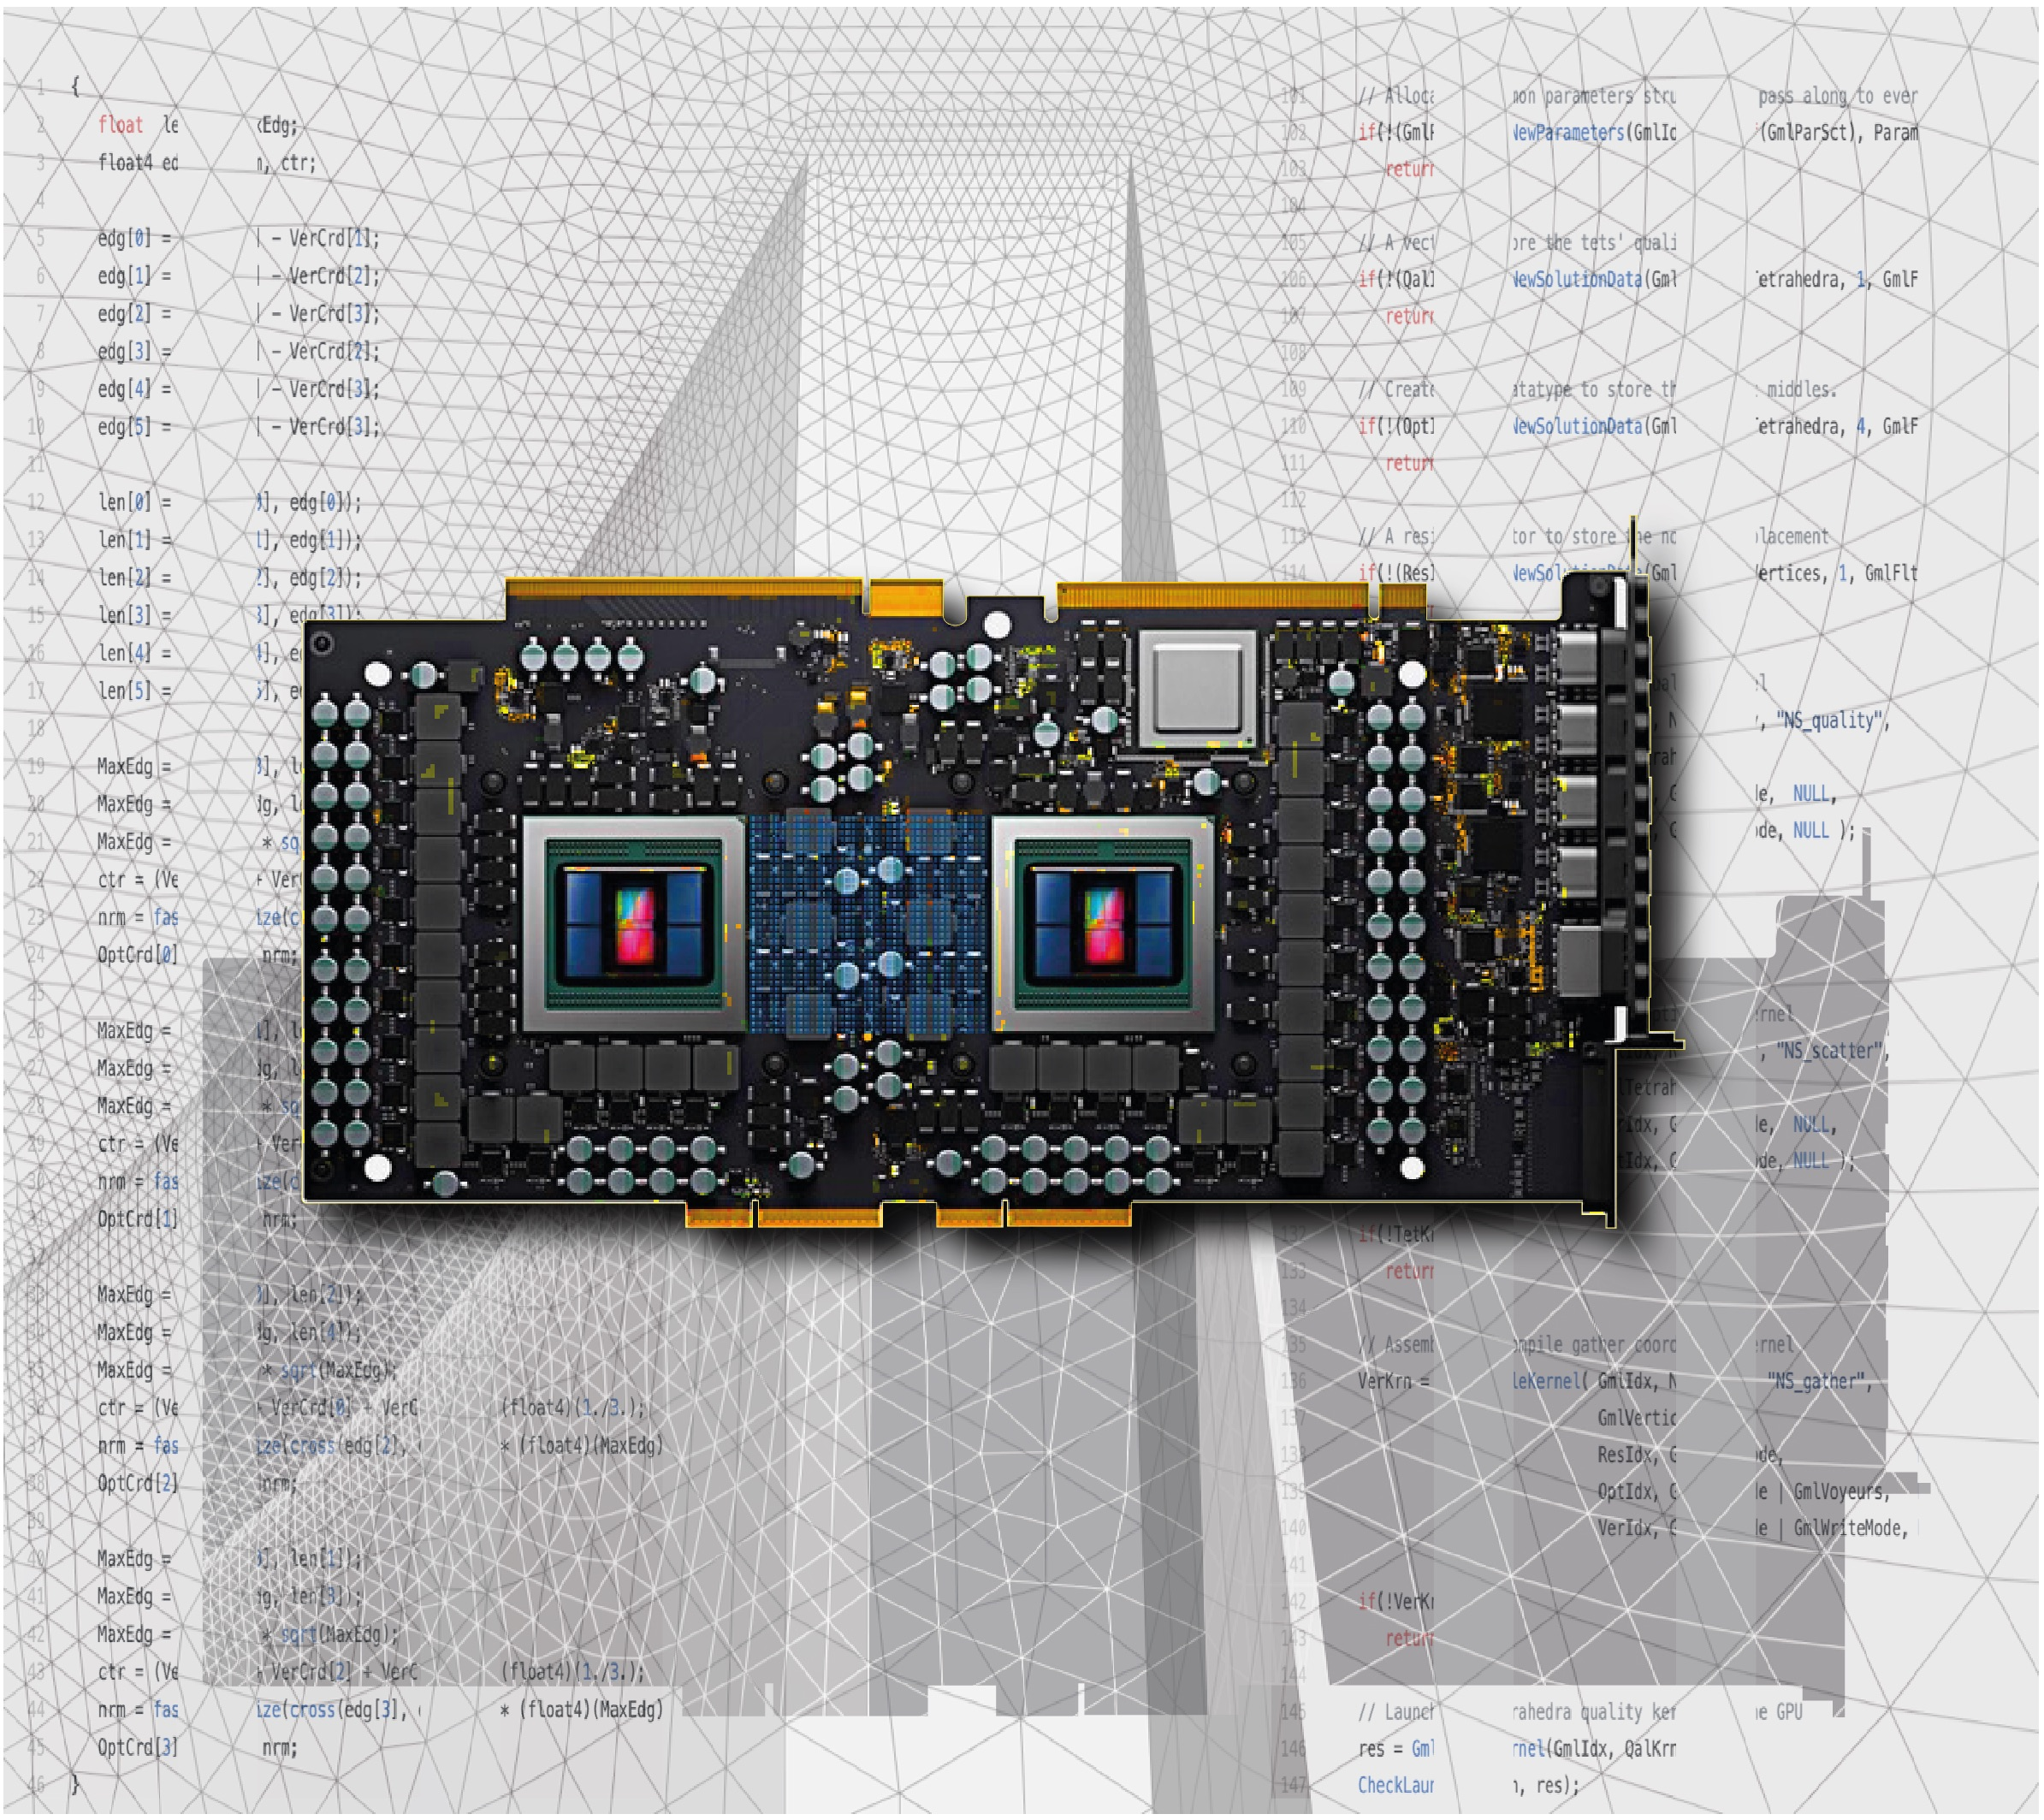
\includegraphics[width=15cm]{gpu.jpg}
\end{center}
\end{figure}

\begin{flushright}
\Large Lo\"ic MAR\'ECHAL / INRIA, Gamma project \\
\normalsize December 2020, document v2.10, library v3.30
\end{flushright}

\end{titlepage}

\clearpage

\setcounter{tocdepth}{2}
\renewcommand*\contentsname{Summary}
\tableofcontents
\vfill

\footnotesize{Cover: original creation from Jean-Luc Maréchal.}
\normalsize

\clearpage


%
%  1 / INTRODUCTION
%

\clearpage

\section{Introduction}
The GMlib v3 aims at easily porting or developing on GPUs any kind of numerical simulation software that deals with unstructured meshes.

It is based on the OpenCL open standard that works on most present systems. The OpenCL not only works with the three major graphic card manufacturers, AMD, Intel and Nvidia, but also on many smaller integrated GPUs present in smartphones, tablets and various embedded devices like those from ARM, Imagination Technologies, etc. Furthermore, in the absence of a dedicated GPU compute devices, OpenCL can generate a multithreaded and vectorized executable quite efficient on multicore CPUs.

But the development of an efficient industrial application on a GPU, that is to say, something more than solving a Laplacian equation on a unit square grid, requires substantial investment in terms of time and competence from the programmer's part.
It is important to note that the most tedious part is the management of data on the GPU, its storage, structure and transfer, that are key factors in the resulting code's efficiency. As for the algorithms, they are not so different from their parallel CPU counterparts, and many software architectures or coding patterns are common to both worlds.

That is why, the GMlib's underlying idea is to abstract as much as possible the handling of data and let the programmer focus freely on the algorithmic part. As the GPU originates from the graphic and video game world, it felt natural to draw inspiration from the most common graphic programming architecture known as \emph{shaders}.

This approach consists in sending all the useful data on the graphic card's memory along with a collection of programs (shaders) to process them. These programs are made of a data access pattern (specifying the data to read or write and how to retrieve it), as well as some mathematical functions to apply to these data. This is the ground architecture of most graphic-oriented libraries like OpenGL, Direct 3D or Vulkan. The GMlib's interpretation of this scheme is to send the mesh's entities to the library (vertex coordinates, elements nodes, etc.) and provide a transparent way to access these mesh data from the user's OpenCL code. Such GPU code, known as a \emph{kernel} in the GMlib's context, is made of a list of mesh entities to be read or write, and the algorithm to execute on these data.

The graphic world concepts like, textures, projections, graphical effects, or normal vectors being replaced by tetrahedra, edges, triangles, as well as the topological links that bind then together like the shells, balls or neighbors information. All these kinds of elements and their relationship are handled and automatically deducted by the GMlib.

On top of that, the GMlib allows the definition of arbitrary storage datatypes made of tables, integers, floats or vectors, for the purpose of storing physical solutions or various flags and tags needed by the algorithms.

Henceforth, a program based on the GMlib unfolds in four steps: initialization of the data structures, setting up of data, compilation of the kernels and execution of the kernels on the GPU.

\clearpage
\paragraph{The initialization and allocation:} the library is first instantiated with a single OpenCL compute device, where the mesh and numerical simulation data structures will be allocated.

\paragraph{Setup the data :} the user has to loop over each entity of each kind to transfer them from its own structures to the library's internal buffers so that they will automatically be stored and transferred to the GPU in the most efficient way.

\paragraph{Compilation of kernels:} each kernel API must be carefully defined before compilation: the main loop mesh kind, the list of datatypes accessed during the loop, and the access mode, either, read, write or both. All this information will be crucial in the way the library will compile the kernel and generates the code that will automatically fetch the required data efficiently. Then the generated kernel source code is compiled into a binary executable that is suited to the run-time hardware (AMD, Intel, NVIDIA).

\paragraph{Execution of the kernels:} once all the data and kernels are transferred to the chosen GPU, it takes only one function call to trigger the execution of a kernel, as many times as needed to converge the simulation scheme, while doing only small interactions between the GPU and the host CPU to modify physical parameters or to get back the residual values and convergence information.


\subsection{Motivation}

Programing on GPUs is interesting in two ways: their performance/price ratio is much higher than that of CPUs and their potential evolution in the foreseeable future is also much brighter than the general-purpose multicore CPUs.

Nevertheless, one should remain realistic as the leader of GPU manufacturing charges a premium price for its high-end HPC products, making a GPU card as costly as a complete CPU-based server. Furthermore, the manufacturers' communication material as well as many scientific papers have boasted extraordinary acceleration factors (two orders of magnitude), comparing GPUs and CPUs in a very unfair way. Most of the time, GPU-based featured examples are working on highly structured data (structured grid meshes in our field of interest) that are well suited to the GPU, and made the comparison against a sequential CPU code. The industrial reality is more complex as it involves unstructured data (tetrahedral meshes) and irregular calculation flow (boundary conditions, convergence criteria), both situations where CPU excels, and adding to that, today's CPUs have up to 64 cores and can scale more than an order of magnitude above sequential code. To make a fair comparison, GPUs and CPUs cost and performance should be evaluated while performing real life simulation codes on unstructured data, using \emph{CUDA} or \emph{OpenCL} on one side, and the \emph{pthread} or \emph{MPI} on the other side. In such case, the GPU over CPU advantage is rather in the vicinity of an order of magnitude, which is good but not great.

In this regard, it is important to pay attention to the development cost, inevitably higher than that of the CPU codes, so that it does not spoil the saving made on the hardware side.
The development on GPUs is more complex for two reasons: the adaptation and transfer of data structures require heavy modifications to meet the very special needs of GPUs vector architecture, secondly, the debugging and optimizing the code is very tedious on GPUs due to their very basic nature and the substantial differences between the different graphic cards.

That is why it is useful to provide developers with an easy to use and efficient framework to port their code on GPUs, but there is no silver bullet to do such porting, whatever some hardware vendors are saying. However, it is possible to develop a dedicated framework for each specific application field like in the numerical simulation domain, where the main data structure is an unstructured mesh that supports all information and is the focus of all calculation. Hence the development of the GMlib that offers an easy and powerful way of storing, transferring and calculating on mesh-based data structures with GPUs.

The development a GPU accelerated software with the GMlib is broken down in two steps:

\begin{itemize}
\item choose one of the featured datatypes that fit your own structures,
\item start from one of the sample codes whose memory access scheme is adequate.
\end{itemize}

Before doing so, you first need to learn how to compile and install the library on your system, which is the topic of the next section.

\subsection{Compile and install}

The library is freely downloadable from the author's GitHub page (cf. \cite{gmlib}) as a single ZIP file that contains all sources, examples and documentation.
It is available under the MIT license (cf. \cite{MIT}), so it can be embedded in any open source or commercial software, in its pristine form or modified, as long as the author is properly cited.

It has been successfully deployed and tested on \emph{Linux}, \emph{macOS} and \emph{Windows10}.
Under macOS, as the OpenCL environment is part of the system, there is no need to install any other component.
It is not the case win Linux and Windows where it is the GPU manufacturer's role to provide the development and runtime software components to execute OpenCL codes.
The three main manufacturers, \emph{AMD}, \emph{Intel} and \emph{Nvidia}, offer free development kits for Linux and Windows that you can find here: \cite{driver_amd}, \cite{driver_intel}, \cite{driver_nvidia}.

The GMlib is made of a main C file {\tt gmlib.c}, the associated header file {\tt gmlib.h}, and should simply be copied into your project source directory and compiled along the way.
In this case, it is your duty to provide the right path to the OpenCL includes and dynamic library, such location can vary depending on the system, hardware and revision.

That is why a CMakefile ({\tt CMakeLists.txt}) is provided as it wraps up the GMlib inside a module that automatically finds the right components at the right place.
All you need to do is the following string of command lines: {\tt cmake .}, {\tt make} and {\tt make install}.
Afterward, you only need to call {\tt find\_package(GMlib)} from your project's CMakefile, to the include the directories with {\tt include\_directories (\$\{GMlib\_INCLUDE\_DIRS\})}, and add the libraries with {\tt target\_link\_libraries(my\_executable \$\{GMlib\_LIBRARIES\})} commands.

There is also an optional external dependency on the {\tt libMeshb} that is needed to compile the examples provided.
It also enables a very useful import/export procedure in the GMlib that will greatly facilitate all mesh I/O based on the INRIA format {\tt *.meshb}.
If you compile both libraries using the included CMakefile, all you need to do is to compile and install the libMeshb first and the GMlib afterward, so that the additional I/O commands will be enabled.
If you prefer to compile both libraries within your own project and Makefile, you just need to pass this additional argument when compiling the GMlib: {\tt -DWITH\_LIBMESHB}.
\medskip

The following files are installed by the CMake file process:

\begin{itemize}
   \item gmlib.a: the static library
   \item gmlib.h: the header
   \item cl2h: a command-line tool that transforms an OpenCl source in a C header file
   \item GMlib\_en.pdf: documentation in English
   \item GMlib\_fr.pdf: documentation in French
   \item examples/: several executable to demonstrate the GMlib's capacities
   \item sample\_meshes/: some mesh files in .meshb format that are used by the demonstration codes
\end{itemize}


%
%  2 / USAGE
%

\section{Usage}

\subsection{API}
\label{sec:API}
Interracting with the library relies on two main elements: datatypes and source codes (i.e. kernels) to process them. Consequently, a software that makes use of the GPU acceleration is a two-step process:
\medskip

\begin{itemize}
\item allocate and setup data like meshes, solution fields and topological links between entities,
\item declare, compile and execute the OpenCL kernels on the GPU.
\end{itemize}
\medskip

Every step and action are executed by the host CPU except for the very last one, the execution of the OpenCL kernel, which is the only part accelerated by the GPU. Talking about \emph{GPU-based software} is a bit far stretched as all input/output, initialization, compilation and post-treatment take place on the host CPU, so it would be more accurate to talk about \emph{hybrid CPU-GPU} or \emph{GPU-accelerated software}. Consequently, it is really important to optimize the CPU time taken by these initial steps as they represent the so-called \emph{Amdahl factor} (cf. \cite{amdahl}) of any GPU-accelerated software.

Incorporating the GMlib in your software starts by initializing a library instance with a single compute device index so that every kernel provided will be compiled and run on this device: {\tt LibIdx = GmlInit(2);}

On the author's laptop computer, such call initializes the library on an AMD Radeon Pro 460 graphic card and returns a unique ID that needs to be provided to any further call the GMlib's procedures. Several instances of the library may run at the same time on different compute devices or even sharing the same one.

As to the present version, only one GPU can be used by a single instance. As a single GPU is made of many cores, known as compute units, and one shared memory space, this kind of concurrent acceleration belongs to the class of \emph{shared memory parallelism}. It is up to the user to distribute the calculation across multiple instances of the library, thus taking advantage of multiple GPUs. The automatic and transparent distribution over multiple GPUs within a single instance is planned for a future version.

Next, you need to define and set up the datatypes to store mesh entities and associated solution fields on the GPU. It introduces a key aspect of the GMlib: the user cannot use its own data containers (tables, structures, objects, etc.) and has to transfer them to the library's internal data structures. It is a strong constraint as a GPU offers only basic structures in order to be efficient and as a result, the job of porting codes to GPUs consists more in adapting the data structures rather than porting the algorithm in the OpenCL language.

Here is a short example to illustrate the process: transfer the mesh's node coordinates from a user's table ({\tt crd[n][3]}) to the library's data structure and create a scalar type to store the speed and a direction vector for each vertex.

\begin{tt}
\begin{verbatim}
VerIdx = GmlNewMeshData(LibIdx, GmlVertices, NmbVer);
for(i=0;i<NmbVer;i++)
   GmlSetDataLine(LibIdx, VerIdx, i, crd[i][0], crd[i][1], crd[i][2], 0);

SpdIdx = GmlNewSolutionData(LibIdx, GmlVertices, 1, GmlFlt, "speed");
for(i=0;i<NmbVer;i++)
{
   speed = rand();
   GmlSetDataLine(LibIdx, SpdIdx, i, &speed);
}

DirIdx = GmlNewSolutionData(LibIdx, GmlVertices, 1, GmlFlt4, "direction");
for(i=0;i<NmbVer;i++)
{
   vector[0] = rand();
   vector[1] = rand();
   vector[2] = rand();
   vector[3] = 0;
   GmlSetDataLine(LibIdx, DirIdx, i, &vector);
}
\end{verbatim}
\end{tt}
\normalfont

Now we wish to iteratively displace these vertices according to their respective direction a speed over a thousand steps and get back the resulting coordinates.
To do so, we first need to create the OpenCL source code to displace a vertex, a so-called \emph{kernel}, and save it in an independent file named {\tt iteration.cl}.
Then we need to compile this kernel and provide it the datatypes' indices, so that the GPU can work on them. In this process, the vertex coordinates are tagged as {\tt GmlReadMode \& GmlWriteMode}, as we need to send them and get them back in the end, and the speed and direction datatypes only need to be transferred once so they are tagged as {\tt GmlReadMode}.

\begin{tt}
\begin{verbatim}
KrnIdx = GmlCompileKernel( LibIdx,  iteration, "iteration", GmlVertices, 3,
                           VerIdx, GmlReadMode | GmlWriteMode, NULL,
                           VitIdx, GmlReadMode               , NULL,
                           DirIdx, GmlReadMode               , NULL );
\end{verbatim}
\end{tt}
\normalfont

A rather long declaration for a very short kernel {\tt iteration.cl}:

\begin{tt}
\begin{verbatim}
VerCrd = VerCrd + VerSpeed * VerDirection;
\end{verbatim}
\end{tt}
\normalfont

This very succinct code brings in a lot of thoughts:

\begin{itemize}
\item There is no iterator that loops over the vertices from 1 to NmbVer,
\item there is no definition of variables at the beginning of the code,
\item there is no access to tables through the loop index to retrieve the vertex data, there is only local data that is already set,
\item in the end, no result is stored in a table,
\item the coordinates, and directions are 3D vectors.
\end{itemize}

\paragraph{Implicit loops:} there is a loop counter that gets incremented from 1 to NmbVer, but the loop iterator is handled by the OpenCL driver and is hidden from the user who has no way to control the loop ordering or stepping. The user can only provide the inner part of the loop, the kernel, and this code snippet is iterated as many times as specified by the main datatype size, in this case, the number of vertices.

\paragraph{Implicit variables:} local variables are automatically defined by the library depending on the parameters given during the kernel compilation. As we asked for access to the vertex coordinates (one 4-float vector per vertex), to the speed (one float per vertex) and direction vector (one 4-float vector per vertex), the GMlib added the right definition before the user's kernel source. As a loop iteration only processes a single vertex at a time, the automatic local variables are big enough to store the data associated with one vertex, hence a scalar and two 4-float vectors. The names of those local variables are automatically set: mesh entities' names are preset (VerCrd, for the coordinates or TriNod for the indices of a triangle's nodes), solution fields' names are constructed depending on the loop context, the main loop entity (here a vertex) is used as a base name, and the user given solution name is concatenated to it, resulting in VerSpeed and VerDirection. 

\paragraph{Access to global tables:} a mesh is made of multiple vertices, yet the library defined a variable to store only one set of coordinates. A global table ({\tt VerCrdTab[ NmbVer ]}, was passed as a global argument to the kernel but was not exposed to the user code and the library generated the proper OpenCL code to read the current vertex's coordinates and store it into a local variable {\tt VerCrd}, the only one accessible by the user. Indeed, when the single kernel code execution begins, the library has already set up and filled the data associated with the current vertex {\tt i}: {\tt VerCrd = VerCrdTab[i]}, {\tt VerSpeed = VerSpeedTab[i]}, {\tt VerDirection = VerDirectionTab[i]}, there is no need to worry about accessing global memory, everything is handled by the GMlib so the user can focus on calculation.

\paragraph{Storage of the results:} as with memory readings, all variables tagged as {\tt GmlWriteMode} at compile time, will be stored in the global tables after the user's kernel calculation. This memory writing is also hidden and transparent. In our example, only the vertex coordinates are accessed in writing mode and the library will add the following line at the end: {\tt VerCrdTab[i] = VerCrd}, so that the updated vertex position is saved in the global GPU memory. Any other calculation results whose datatype was not properly tagged as writable will be lost at the end of the loop iteration !

\paragraph{Vector calculation:} the OpenCL language features vector extensions of every scalar type, with size 2,4,8 and 16 available, and uses the \emph{operator overloading} technique from the C++ to adapt the calculation to the variable's type. Their prototype if straightforward as it adds the vector size after the name string: {\tt float4} defines a four entries floating point vector or {\tt int16} for a sixteen-entry integer vector. In our kernel, the {\tt VerCrd} and {\tt VerDirection} are 3D vectors (stored on a float4 for padding consideration) and the operation {\tt VerCrd = VerCrd + VerDirection} triggers a vector operation adding all four components in one go. So what happens when the speed, which a scalar, is multiplied by the direction, which is a vector ? Here again, the OpenCL compiler detects the case and chooses the right scalar vector multiply instruction.


\subsection{Datatypes}

The user being constrained to use only the provided datatypes, it is very important to fully understand their usage, capacity and limitation. These types fall into three categories:

\begin{itemize}
        \item mesh datatype: vertices, edges, triangles, etc,
        \item free solution fields: additional information related to one kind of mesh datatype and made of scalar, table or vectors of integers or floats,
        \item topological links: a table that links every entity of one mesh kind to an arbitrary number of entities from another kind, for examples, linking vertices to the ball of surrounding triangles, or a neighbor’s table linking tetrahedra sharing a common triangle.
\end{itemize}

\paragraph{Mesh datatypes:} they are made for storing any kind of first order mesh entities (high order elements are scheduled for a future version). The most common kinds of finite elements are available: Vertices, Edges, Triangles, Quadrilaterals, Tetrahedra, Pyramids, Prisms et Hexahedra. Elements are made of a simple list of node indices stored as integers, plus an additional integer to store a physical reference. Vertices are made of a vector of four floats, the last one being ignored, and an integer to store a reference. Allocating a mesh datatype is done with the help the {\tt GmlNewMeshData()} procedure, providing only the kind tag (GmlVertice, GmlEdges, etc., cf gmlib3.h) and the number of lines to allocate. Setting up the data is done with the procedure {\tt GmlSetDataLine()}, giving it the datatype, the line number (from $0$ to $n-1$) and a variable list of arguments whose number and types depend on the mesh kind. The following example simply allocates and set up a mesh made of three vertices.

\begin{tt}
\begin{verbatim}
VerIdx = GmlNewMeshData(LibIdx, GmlVertices, 3);
GmlSetDataLine(LibIdx, VerIdx, 0, 1.5, 2.3, 1.0, 8);
GmlSetDataLine(LibIdx, VerIdx, 1, 9.2, 8.3, 1.0, 6);
GmlSetDataLine(LibIdx, VerIdx, 2, 6.3, 1.6, 2.3, 0);
\end{verbatim}
\end{tt}
\normalfont

Word of caution: all tables use the C convention and range from $0$ to $n-1$.

\paragraph{Solution fields:} it is basically a free datatype that you can define to suit your needs. It can be made of bytes, integers, floats or doubles, in scalar or vector form (sizes 2,4,8 or 16), and gather them into a one-dimensional table of arbitrary size. For example, a solution can range from a single scalar integer ({\tt int scalar}), to a table of five integer vectors of size eight ({\tt int8 table[5]}). There are only two limitations:
\medskip

\begin{itemize}
        \item A solution datatype must always be related to a single mesh datatype, consequently, you cannot specify the number of lines of the global solution table as it is inherited from its base mesh datatype. Access to the solution datatype is always made through the topological link of its supporting mesh kind (see topological links below).
        \item You cannot mix different types in one field like with a C structure that can mix integers, floats, etc. To do so, you have to define two separate solution fields, each made of a single OpenCL type.
\end{itemize}
\medskip

The allocation is made with the {\tt GmlNewSolutionData()} procedure, specifying the reference mesh kind, the size of the local table (or 1 if you only need a single value), followed by the GMlib's predefined type (GmlByte, GmlInt16, GmlFloat4, etc.) and finally a string containing the name that will be used by the kernel source code generator in order to identify and access this data. The data can by set with the {\tt GmlSetDataLine()} procedure, like any mesh datatype, except that instead of passing a separate argument for each entry, a pointer to a table containing all entries must be given and its content will be copied to the library's internal buffer. The following example allocates and set up a local table made of two floats that is associated to the vertex datatype previously defined:

\begin{tt}
\begin{verbatim}
float vec[2];
VecIdx = GmlNewSolutionData(LibIdx, GmlVertices, 2, GmlFlt, "WeightSpeed");
vec = {1.2, -6.3};
GmlSetDataLine(LibIdx, VecIdx, 0, &vec);
vec = {0.3,  5.2};
GmlSetDataLine(LibIdx, VecIdx, 1, &vec);
vec = {3.4, -0.1};
GmlSetDataLine(LibIdx, VecIdx, 2, &vec);
\end{verbatim}
\end{tt}
\normalfont

\paragraph{Topological links:} it is the most powerful datatype but also the most complex to understand and manipulate. With some imagination and cunning tricks, it is possible to circumvent most GPU's limitations through these links. A topological link is a table that binds two datatypes, the first one being the source and the other one being the destination. For each source entity, it stores one or several entities of the destination type. For example, the source maybe the triangles table, the destination may be the tetrahedra table, and the line size could be two entries, enough to store for each triangle the two neighboring tetrahedra sharing a common face.

Links are one way, inverting the datatype in the previous case would result in a different topological table, for each tetrahedron, it would state the four potential triangles sharing each of the tetrahedron's face. This topological links are used to access data in indirect memory access kernels (see section \ref{sec:kernels_indirects}) as they enable the access of data related to tetrahedra while performing a loop on triangles, to keep on with our example.

One of the GMlib key point is that every possible link between any two kinds of mesh entities is automatically built when required at kernel compile time. For example, if one wants to loop over edges and needs to read some data associated with the triangles, the library will automatically build the \emph{triangle shell} of edges which is the list of triangles that share the same edge.

Beyond these implicit tables, the user can create any kind of topological table to enable some special purpose memory access and override the default path, for instance, in the case of edges pointing to triangles, you may instead need a list of only two triangles pointing to the \emph{upwind} and \emph{downwind} elements, as you are developing a flow solver and you don't need an edge's triangles shell. To do so, it would take to allocating a link with {\tt GmlNewLinkData()}, stating that the source is the edges, the destination is the triangles and the size is two. Following the allocation, you can set up the table with the general-purpose procedure {\tt GmlSetDataLine()} giving for each line the link index, the edge number and a pointer to a local table containing the two triangles indices. The size, nature and meaning of a link is up to you, you might want to build the list of the 180 geometrically closest pyramids from any vertex if needed !
That is easily said and done:

\begin{tt}
\begin{verbatim}
int pyramids[ NmbVer ][ 180 ];
PyrIdx = GmlNewLinkData(LibIdx, GmlVertices, GmlPyramids, 180, "PyrTab");
for(i=0;i<NmbVer;i++)
   GmlSetDataLine(LibIdx, PyrIdx, PyrTab[i]);
\end{verbatim}
\end{tt}
\normalfont

Remark: the reverse link would have a pyramid pointing to vertices, which is nothing more than the table of pyramids' nodes itself. By the way, the elements tables could be considered as topological links between elements and vertices.

\subsection{Direct memory access kernels}
\label{sec:kernels_directs}
It is the most basic kind of kernel, it loops over the elements of a single kind of mesh entity and reads or writes only datatypes associated with this kind. If a kernel loops over the vertices and reads a solution field associated to each vertex, this solution table is accessed directly using the loop counter. While processing the vertex number $i$, any table is accessed through $table[i]$, hence the name direct memory access kernel. This the most efficient access pattern as it allows the GPU to prefetch memory before it is needed by the calculation, thus reaching up almost 100\% of the theoretical bandwidth.

In the introducing example (\ref{sec:API}), the two solution fields allocated, Speed and Direction, are related to the vertices, so the kernel looping over vertices and adding the $Speed * Direction$ will read the coordinates, speed and direction tables in a consecutive way.

\begin{tt}
\begin{verbatim}
VerCrd = VerCrd + VerSpeed * VerDirection;
\end{verbatim}
\end{tt}
\normalfont

In this single line kernel, at each iteration of the loop, ranging from $0$ to $NmbVer-1$, the coordinate vector, speed scalar and direction vector are read from the global tables and stored to local variables by the library. Behind the scenes, the GPU accesses memory with a 32-byte or 64-byte word size, so several vertex coordinates are fetched with a single memory operation and stored into the GPU's cache, the next loop iterations will just have to search the cache for the previously read data.

In such situation, the automatic naming convention for the local variables accessible to the user within the kernel code is straightforward: it is the concatenation of the loop mesh kind and the name of the data being accessed. For the mesh datatypes the name is preset by the library in the gmlib.h file as a trigram to make names shorter (Ver, Edg, Tri, Qad, Tet, Pyr, Pri, Hex), for the solution datatypes it is the name given by the user at allocation. In our example, as the kernel loops over vertices (full name: {\tt GmlVertices}, short name: {\tt Ver}) and accesses the coordinates (short name: {\tt Crd}), the speed (named {\tt Speed} set by the user) and {\tt Direction}, the library will automatically define and sets these local variables: {\tt VerCrd}, {\tt VerSpeed} and {\tt VerDirection}, elementary !

Remark: a direct access pattern allows for read, write, or read \& write memory access without restriction.

\subsection{Indirect memory access kernels}
\label{sec:kernels_indirects}
a kernel is called indirect when it accesses table entries through an index that is different from the main loop index. In such case, an indirect memory access looks like {\tt a = u[v[i]]}, while a direct access is {\tt a = u[i]}. This kind if indirect access is slower for two reasons.

First of all, it takes two memory reads to get a single value of interest as the GPU first reads the indirection index in a temporary data, {\tt tmp = v[i]}, then reads the useful one, {\tt a = u[ tmp ]}.

Second and most important reason, while reading the indirection indices is consecutive in memory, {\tt j = v[i]} is next to {\tt k = v[i+1]}, this not the case with the indirect locations, {\tt u[j]} and {\tt u[k]}, as the index $i$ and $j$ are unrelated. Consequently a full cache-line is read from the memory when accessing each indirect value, making for poor utilization of the theoretical bandwidth.

Two technics can be used to tackle this problem, first the mesh can be renumbered through an \emph{SFC} (Space Filing Curve) like Hilbert (cf. \cite{peano_hilbert}) in order to increase the cache hit, second, using vectorized types, which are much faster than scalar access on GPUs, to store the meshing data (the four nodes of a tetrahedron are stored in an int4 vector and the eight hexahedra around vertex balls are stored either in an int8 or an int32 depending on the vertex degree). All this renumbering and vector storage is done via the provided command-line program \emph{hilbert} in the utility’s section.

Let's analyze an example to illustrate this indirection process: a kernel loops over the triangles ({\tt Tri}) that are made of vertices ({\tt Ver}) and needs to access their coordinates ({\tt Crd}). The library will automatically initialize and set up a table containing the three nodes indices ({\tt int TriVer[3]}) as well as three vectors containing their coordinates ({\tt float4 TriCrd[3]}). Here is a simple code looping over the triangles and computing the barycenter:

\begin{tt}
\begin{verbatim}
KrnIdx = GmlCompileKernel( LibIdx,  barycenter, "center", GmlTriangles, 3,
                           VerIdx, GmlReadMode , NULL,
                           TriIdx, GmlReadMode , NULL,
                           BarIdx, GmlWriteMode, NULL );
\end{verbatim}
\end{tt}
\normalfont

And the associated kernel:
\begin{tt}
\begin{verbatim}
center = (TriCrd[0] + TriCrd[1] + TriCrd[3]) / 3.;
\end{verbatim}
\end{tt}
\normalfont

The return variable ({\tt center}) is a single float4 vector as it is related to the triangle datatype which is the kernel main loop entity. On the contrary, the {\tt TriCrd} variable is a three entries table as it is related to the vertices and a triangle is made of three of them.

As you can see, accessing the triangle's nodes indices to get their coordinates is unnecessary as the library has automatically filled the local coordinates table before executing the user's kernel code. The indirection from the triangle's nodes indices to the nodes coordinates went through a topological link which is a hidden process. What may be unsettling in the beginning is that the same datatype accessed indirectly from two kernels with different main loop entities will be defined in a different way. For instance, replacing the {\tt GmlTriangles} type with the {\tt GmlEdges} type in this example results in the coordinates table to change from {\tt float4 TriCrd[3]} to {\tt float4 EdgCrd[2]} ! In the second case, the coordinates are those from the edge's nodes, hence the automatically generated name {\tt EdgCrd}, and as its indirection goes through an edge nodes, it is defined as a table with two entries instead of three when accessed via a triangle. That why we talk about \emph{context based automatic naming}. Once you get confident with this automatic naming and setup, you can access any kind of data, either mesh entities or solution fields, regardless of the main loop datatype, as all possible links between any pair of entities is handled by the GMlib.

\paragraph{Topological link categories, downward, transverse and upward:} a link is called downward (i.e. a downlink) if the source entity is of higher dimensions as the pointed one, for instance, when triangles point to edges. It is called transverse when the two kinds belong to the same dimension, even though they may not be exactly the same kind, for example triangles pointing to neighboring quadrilaterals. Likewise, it is called an uplink when the source entity is of lower dimensions than the destination one, like the vertex's ball that links a vertex with an arbitrary number of tetrahedra. Let's review each link's properties.

\paragraph{Downlinks:} this is the most trivial one, it happens when a kernel loops over an element kind and accesses data associated with its nodes. In this case, the downward topological link is simply the mesh elements table that lists each element's nodes. The library does not need to build any intermediary information, it simply transfers the elements table to the GPU. Such link is rather efficient in terms of memory access as the number of nodes for each element is a constant value stored in a power of 2 vector.

\paragraph{Transverse links:} the second category is a little bit more subtle as the default link used by the library is the identity. Accessing triangles while performing a loop on triangles means no indirection at all, in this case the kernel is a basic direct access one as seen in the section \ref{sec:kernels_directs}. But the user may override this default direct access by providing his own tailor-made topological table that could link triangles between themselves in a different way for example, providing the list of the three possible neighbors for each triangle. In this case, the kernel is transverse, as the main loop entity and the accessed entity are the same, but it is not a direct link as the library needs to go through the neighbor’s table to access their related data. Here is an example to illustrate this case: as the previous example calculated the triangle barycenter, now we ant to search for each triangle which of its three neighbors' center is closest from it own.

\begin{tt}
\begin{verbatim}
NgbIdx = GmlSetNeighbours(LibIdx, GmlTriangles);
DisIdx = GmlNewSolutionData(LibIdx, GmlTriangles, 1, GmlFlt, "min_dist");
KrnIdx = GmlCompileKernel( LibIdx,  distance, "distance", GmlTriangles, 2,
                           BarIdx, GmlReadMode , NgbIdx,
                           DisIdx, GmlWriteMode, NULL );
\end{verbatim}
\end{tt}
\normalfont

The first line creates a topological link that gives the three possible neighbors for each triangle. The {\tt GmlSetNeighbours()} procedure automatically builds the connectivity, allocate the topological datatype and set it up. The returned link index is passed as an argument associated to the barycenter table index: {\tt BarIdx, GmlReadMode , NgbIdx} to override the default access. Without this argument, as the kernel loops over the triangles and the barycenters are associated with the same entity, the library would simply read the barycenter of the triangle being processed during each loop iteration, so {\tt float4 VerCenter} would be defined. By providing a special purpose table that links each triangle to possibly three other ones, the library creates a local table with four entries, the first one for the triangle being processed itself, and the next three for its potential neighbors: {\tt float4 TriCenter[4]}. Here is the corresponding kernel:

\begin{tt}
\begin{verbatim}
float d1, d2, d3;
d1 = distance(TriCenter[0], TriCenter[1]);
d2 = distance(TriCenter[0], TriCenter[2]);
d3 = distance(TriCenter[0], TriCenter[3]);
min_dist = min(d1, d2);
min_dist = min(min_dist, d3);
\end{verbatim}
\end{tt}
\normalfont

Here, the centers table is named {\tt TriCenter[4]} as the loop entity is the triangle (short name {\tt Tri}) and the accessed data were named {\tt Center} by the user. The first entry {\tt TriCenter[0]} is the barycenter of the triangle being processed and the three others are its neighbors barycenters. Note that a neighbor index might by $0$ if the corresponding edge is on the mesh boundary, in this case, the center is initialized with zeros ${0,0,0}$. To take this case into account, it is useful to check the element's degree variable that is set by the library when dealing with indirect accesses ({\tt int TriDeg}) which indicates the number of non-null neighbors for each triangle. In every indirect kernel, such variable whose name is made of the loop entity short name concatenated to {\tt Deg}, is always set to indicate the degree of the entities. Dor example, the number of triangles in the ball of a vertex (ranging from 0 to 32) or the number of tetrahedra on each side of a triangle (ranging from 0 to 2).

\paragraph{Upward links:} or uplink, this is the most complex one as its size is varying with each loop entity. And dynamic sizing is something inefficient on GPUs that favor constant sizes padded on power of 2. Indeed, as the number of nodes pointed by a triangle is always three and can be stored in an int4 vector, the reverse link, the number triangles sharing a common vertex is not a constant in an unstructured mesh as it is varying from 1 to infinity (the value of infinity has been limited to 32 in the case of the vertex ball of triangles).

In order to process these cases efficiently, a complex system is used beneath the scene by the GMlib. First of all, renumbering the mesh through the provided Hilbert command line is necessary. Its purpose is to sort out vertices according to their degree, the lower degree vertices being stored first and the higher degree ones being moved to the table's end. In the case of vertices pointing to triangles, the lower degree threshold is set to 8 and the maximum higher degree to 32. Consequently, the GMlib splits the topological table linking vertices to triangles into two separate tables: the first one stores the triangle indices in an int8 vector (some elements indices can be $0$ if a vertex degree is lower than 8), and a (hopefully) shorter table with int32 vectors. When a kernel looping over vertices and accessing the triangles-related data is executed, the library runs the kernel in two steps, the first time with the low degree table and a second time with the high degree table. The whole process is transparent and the only thing noticeable to the user is the automatic variable ({\tt VerTriDeg} in this case) storing the degree that varies with each iteration.

Remark: a variable accessed indirectly through an uplink can be $0$, as the variable size tables are padded to the nearest power of 2 vector and consequently, some entries are initialized with null values.

Let's go back to the triangles' barycenter example, but this time we would like to loop over the vertices, access the barycenters of the vertex ball of triangles, compute the average value and relax the vertex coordinates toward this value (a kind of vertex smoother).

\begin{tt}
\begin{verbatim}
CrdIdx = GmlNewSolutionData(LibIdx, GmlVertices, 1, GmlFlt4, "relaxed");
KrnIdx = GmlCompileKernel( LibIdx,  smoothing, "smoothing", GmlVertices, 2,
                           BarIdx, GmlReadMode , NULL,
                           CrdIdx, GmlWriteMode, NULL );
\end{verbatim}
\end{tt}
\normalfont

The upward link from vertices to triangles does not need to be specified and the link argument is set to NULL as we are using the default link between these two datatypes called the vertex ball of triangles.

Here is the OpenCL kernel that sums all triangles' center and relaxes the vertex toward this new position:
\begin{tt}
\begin{verbatim}
int i;
float4 NewCrd = {0};
for(i=0;i<VerTriDegMax;i++)
  NewCrd += VerTriBar[i];
relaxed = 0.8 * relaxed + 0.2 * NewCrd / VerTriDeg;
\end{verbatim}
\end{tt}
\normalfont

An upward access kernel defines an additional variable to provide the loop entity degree at each iteration, in this case, how many triangles are pointed by a vertex ball: {\tt VerTriDeg}. You may notice that the last kernel line divides the barycenters' sum by this degree in order to get the mean value. The inner loop that sums all triangles' centers could also use this counter but it would be really slow as a GPU performs poorly when a loop count is unknown at compile time. To circumvent this limitation, another automatic variable related to the vertex degree is set: {\tt VerTriDegMax}, this is the vector size that contains each vertex ball of triangles. In the first iterations of the loop, this value is a constant set to 8, and climbs to 32 during the last lines that deal with the high degree vertices. We choose to loop up to this maximum value and not the real vertex degree, thus adding some null coordinates to the average value and the consequence is a faster execution ! Why so ? Because the value {\tt VerTriDegMax} is known at compile time and the OpenCL compiler can generate a fully optimized code. Note that the mathematical result is unaffected as we are adding null values to the sum and in the end, it is divided by the right value {\tt VerTriDeg}.


\subsection{Pair of scatter-gather kernels:}
A problematic common to all concurrent programming schemes, either distributed parallelism, multithreading or GPU computing is the concurrent indirect memory writes. It is the case when one wants to loop over elements and write some data associated with their vertices. In such situation, two concurrent compute units processing different elements could write at the same time and at the same vertex position because separate sets of elements might share some common vertices.

The most common way to address this problem is to split a single indirect memory writes loop into two separate loops known as a \emph{scatter} loop and a \emph{gather} loop. With this technic, the resulting two loops are performing indirect memory reads, and direct memory writes, thus eliminating the memory write consistency.

Let's start with a kernel that loops over the triangles, computes some value and needs to add it to a vertex-related field. This single loop performs indirect memory writes, so it needs to be split in the two following scatter-gather loops, each in a dedicated kernel.

The scatter kernel, will loop over the triangles, perform the calculation and store it in a temporary field associated with the triangles. This new loop does only direct memory writes.

The gather kernel will loop over the vertices, read the previously set temporary field associated with the triangles (an indirect memory read), sums up all local contributions and write the result to the final vertex-related field. Like the scatter kernel, this new one only performs direct memory writes.

These two loops are not really independent, they just execute a part of the real loop, the first one scattering partial results to triangles' data and the second one gathering all the local data into the final vertex data. Hence the name \emph{scatter gather}.


Compiling the \emph{scatter} kernel:
\begin{tt}
\begin{verbatim}
TmpIdx = GmlNewSolutionData(LibIdx, GmlTriangles, 1, GmlFlt4, "Tmp");
KrnIdx = GmlCompileKernel( LibIdx,  scatter, "scatter", GmlTriangles, 3,
                           VerIdx, GmlReadMode , NULL,
                           TmpIdx, GmlWriteMode, NULL );
\end{verbatim}
\end{tt}
\normalfont

OpenCL code of the \emph{scatter} kernel:
\begin{tt}
\begin{verbatim}
Tmp = (TriCrd[0] + TriCrd[1] + TriCrd[3]) / 3.;
\end{verbatim}
\end{tt}
\normalfont

Compiling the \emph{gather} kernel:
\begin{tt}
\begin{verbatim}
SolIdx = GmlNewSolutionData(LibIdx, GmlVertices, 1, GmlFlt4, "VerSol");
KrnIdx = GmlCompileKernel( LibIdx,  gather, "gather", GmlVertices, 2,
                           TmpIdx, GmlReadMode , NULL,
                           SolIdx, GmlWriteMode, NULL );
\end{verbatim}
\end{tt}
\normalfont

OpenCL code of the \emph{gather} kernel:
\begin{tt}
\begin{verbatim}
int i;
float4 NewSol = {0};
for(i=0;i<VerTriDegMax;i++)
  NewSol += VerTriTmp[i];
VerSol = NewSol / VerTriDeg;
\end{verbatim}
\end{tt}
\normalfont


\subsection{OpenCL programming}
A full course on OpenCL programing or even a short description would be out this document's scope. The reader should better refer to the official Khronos Group documentation \cite{khronos}, a non-profit organization that publishes open standards. Furthermore, GPUs hardware manufacturers also publish various materials on the subject: courses, best practices and examples, and their developer's web pages are treasure troves (cf. \cite{nvidia}, \cite{gpuopen}, \cite{rocm} and \cite{apple}) for that matter.


%
%  3 / COMMANDS
%

\section{List of procedures}

\subsection{GmlCheckFP64}
Check for the presence of double precision floating point extension. The OpenCL standard makes the presence of 32-bit compute units mandatory, but half-precision (16-bit) and double precision (64-bit) capabilities are optional and should be checked at runtime.

\subsubsection*{Syntax}
{\tt flag = GmlCheckFP64(LibIdx);}

\subsubsection*{Parameters}
\begin{tabular}{|m{2cm}|m{1.5cm}|m{10.5cm}|}
\hline
Parameter  & type    & description \\
\hline
LibIdx     & size\_t & instance index as returned by GmlInit() \\
\hline
\end{tabular}

\medskip

\begin{tabular}{|m{2cm}|m{1.5cm}|m{10.5cm}|}
\hline
Return     & type   & description \\
\hline
flag       & int    & 0: no 64-bit FP capability available, 1: 64-bit FP available \\
\hline
\end{tabular}

\subsubsection*{Comments}
Even though most today GPUs, including video-game cards, feature double precision units, their number is often 1/32th to 1/4th of the number of single precision units, making 64-bit calculations as many times slower. Consequently, the GPU 64-bit Gflop/s might even be lower than that of the main CPU ! In such case, the FP64's availability might be deceitful.


\subsection{GmlCompileKernel}

\subsubsection*{Syntax}
{\tt KrnIdx = GmlCompileKernel(LibIdx, OclSrc, PrcNam, MshTyp, NmbDat, ...);}

It's certainly the most complex GMlib's procedure !

Its purpose is to build a binary executable suitable for the selected graphic card. Its inputs are an ASCII OpenCL source, a main loop mesh element type and a list of datatypes to be accessed in read or write mode, directly or indirectly. The main parameter is the kind of mesh element to loop over as it will determine the access mode of the flowing datatypes, either mesh entities or solution fields. The next parameter is the number of such datatypes and for each of them, the memory access mode and specific options should be given as follows.

First, the index of each datatype must be given. The memory access pattern, direct or indirect, is deduced from a 2D topological-link table, one entry being the loop element kind and the second one being the accessed element kind.

In the case where both entries belong to the same geometrical dimension, the access pattern is direct and the user's data will be made of a single value: for example, if one loops over triangles and wants to access to a field containing each triangle's normal, the corresponding generated value will be of type {\tt float4 TriNrm} because each loop iteration processes a single triangle and each triangle has only one normal vector associated that is stored in a single {\tt float4} value.

In the case where the accessed mesh entity is of lower geometrical dimension than the loop element kind, we are talking about a \emph{downlink kernel}, the accessed data will be presented in a local table whose size will be that of the number of pointed entities that make up a single main loop element entity. For example, if one loops over triangles and wants to access to normal vectors associated with each of the triangle's vertices, as there are three vertices per triangle, the local value will be defined as such: {\tt float4 TriVerNrm[3]} because there are three vertex normals per triangle.

In the case where the accessed mesh entity is of higher dimensions as that of the main loop entity, we are talking about an \emph{uplink kernel} (such as a vertex's ball or an edge's shell), here again, the pointed data will be stored in a local table whose size will be varying at each main loop iteration according to the processed entity's degree. Let's say that this time one wants to loop over the vertices and access each of the vertex's ball of triangles' normal vector (the other way around as the previous example), the local value will be defined as such: {\tt VerTriNrm[ VerTriDeg ]}, and the {\tt VerTriDeg} will be defined appropriately for each vertex.

Furthermore, it is possible to bypass the default topological link provided by the connection table and give its own tailor-made link table, to give element neighbors for instance. If one wants to loop over tetrahedra and access to some fields associated to the processed element but also to the other ones sharing a common triangle (its neighbors), it is possible to generate such neighbors table with the procedure {\tt GmlSetNeighbours()} and pass it along during the kernel creation as a dedicated link associated with the tetrahedra mesh entity.

The following example illustrates the differences between all these access patterns by accessing to the same datatype but in a different context. Let's start with a mesh made of vertices, triangles, tetrahedra and a field associated with each triangle to store its area. One would like to read each triangle's area while looping over their vertices in a first kernel, then over tetrahedra in a second one, over the triangle themselves in a third one, and finally, over the triangles and their neighbors. You will notice that the same kind of data (a single scalar value containing the triangle's area) will be defined and accessed in a completely different way in each kernel !

\subsubsection*{Parameters}

\begin{tabular}{|m{2cm}|m{1.5cm}|m{10.5cm}|}
\hline
Parameter  & type    & description \\
\hline
LibIdx     & size\_t & instance index as returned by GmlInit() \\
\hline
OclSrc     & char *  & pointer on a character string containing the kernel OpenCL source to compile \\
\hline
PrcNam     & char *  & pointer on a character string containing the procedure name as it will appear in the generated kernel \\
\hline
MshTyp     & int     & mesh datatype on which the kernel will loop: this information is crucial as it will determine the access pattern to all users’ data in the kernel \\
\hline
NmbTyp     & int     & number of datatypes that will be read and/or written by the kernel, for each data the three following arguments are expected: \\
\hline
DatIdx     & int     & index of the datatype to access \\
\hline
flags      & int     & a list of flags concatenated with the logical operator \emph{OR}, represented by of vertical bars ({\tt |} in C, such as {\tt GmlReadMode}, {\tt GmlWriteMode}, {\tt GmlRefFlag} and {\tt GmlVoyeurs} \\
\hline
LnkIdx     & int     & index of a topological link type to follow in order to access the datatype, if this value is nought, the library will take the default built in link. \\
\hline
\end{tabular}

\medskip

\begin{tabular}{|m{2cm}|m{1.5cm}|m{10.5cm}|}
\hline
Return     & type   & description \\
\hline
DatIdx     & int    & index number identifying the new kernel \\
\hline
\end{tabular}


\subsection{GmlDebugOff}
Disable the debug mode (default status).

\subsubsection*{Syntax}
{\tt GmlDebugOff(LibIdx);}

\subsubsection*{Parameters}

\begin{tabular}{|m{2cm}|m{1.5cm}|m{10.5cm}|}
\hline
Parameter  & type    & description \\
\hline
LibIdx     & size\_t & instance index as returned by GmlInit() \\
\hline
\end{tabular}


\subsection{GmlDebugOn}
Turn on the debug mode which will print out the complete generated source listings, including the hidden declarations, and the memory reading and writing code blocks added by the library.

\subsubsection*{Syntax}
{\tt GmlDebugOn(LibIdx);}

\subsubsection*{Parameters}
\begin{tabular}{|m{2cm}|m{1.5cm}|m{10.5cm}|}
\hline
Parameter  & type    & description \\
\hline
LibIdx     & size\_t & instance index as returned by GmlInit() \\
\hline
\end{tabular}


\subsection{GmlDownloadParameters}
Copies the parameters structure's content, as defined with  {\tt GmlNewParameters()}, from the GPU mem to the host CPU so that any information written by the kernel during execution can be exploited.

\subsubsection*{Syntax}
{\tt GmlDownloadParameters(LibIdx);}


\subsection{GmlEvaluateNumbering}
Returns a synthetic numbering evaluation factor of mesh entities in terms of cache memory access hit. The closer to 100\% is the value, the more likely the memory accesses will hit the cache instead of the slower graphic memory. Conversely, a value close to 0\% indicates that the mesh was not properly renumbered through an \emph{SFC} (cf. \cite{peano_hilbert}) and the kernel execution will be inefficient because of too many accesses to the graphic memory will be needed (they are usually two orders of magnitude slower than the cache memory).

\subsubsection*{Syntax}
{\tt efficiency = GmlEvaluateNumbering(LibIdx);}

\subsubsection*{Parameters}
\begin{tabular}{|m{2cm}|m{1.5cm}|m{10.5cm}|}
\hline
Parameter  & type    & description \\
\hline
LibIdx     & size\_t & instance index as returned by GmlInit() \\
\hline
\end{tabular}

\medskip

\begin{tabular}{|m{2cm}|m{1.5cm}|m{10.5cm}|}
\hline
Return     & type   & description \\
\hline
efficacité & float  & returns the cache hit efficiency in percent (\emph{cache hit}) \\
\hline
\end{tabular}

\subsubsection*{Comments}
the coefficient is evaluated by simulating a loop over every element of every kind while accessing to their vertices. In order to compute a numerical value, an imaginary cache memory whose size is around that of real GPUs is used. Consequently the returned value is only an approximation.


\subsection{GmlExtractEdges}
This procedure builds the list of unique edges present in the volume mesh. To do so, it parses all mesh entities of dimension 1 (edges), 2 (faces) and 3 (volumes) to extract all their edges add them to the list. If an edge list was already present before calling this procedure, to specify the sharp edges for example, the former list entries are copied to the new list and newer edges will be added at the end of the list. After this step, the former list is freed and the new datatype index containing the new edge list is returned ({\tt NewEdgIdx = GmlExtractEdges(LibIdx)}).

\subsubsection*{Syntax}
{\tt DatIdx = GmlExtractEdges(LibIdx);}

\subsubsection*{Parameters}
\begin{tabular}{|m{2cm}|m{1.5cm}|m{10.5cm}|}
\hline
Parameter  & type    & description \\
\hline
LibIdx     & size\_t & instance index as returned by GmlInit() \\
\hline
\end{tabular}

\medskip

\begin{tabular}{|m{2cm}|m{1.5cm}|m{10.5cm}|}
\hline
Return     & type   & description \\
\hline
DatIdx     & int    & index number of the new edges table \\
\hline
\end{tabular}

\subsubsection*{Comments}
The numbering of the edges table generated this may be suboptimal as the edges are generated by parsing the elements in consecutive order, consequently, the edge numbering roughly follows that of volume elements and inherit their renumbering in some way. Such inheritance will never be as optimal as if the edges table was properly renumbered through an SFC like Hilbert. Furthermore, these edges are not sorted against their uplink degrees (number of incident face or volume elements) and will take more GPU memory as most of the uplink tables will be stored in the high-count area.

For example, if edges are extracted from tetrahedra in this way, most of the shell tables will take 32 entries (the maximum number of tetrahedra allowed to share a common edge) while the average is 6. In such a situation, renumbering the edges and sorting then against their degrees through a Hilbert curve should be considered if one wants to perform an uplink kernel that loops over the edges and accesses their shell of tetrahedra.


\subsection{GmlExtractFaces}
This procedure builds the list of unique faces present in the volume mesh. To do so, it parses all mesh entities of dimension 2 (faces) and 3 (volumes) to extract all their faces add them to the list. If a triangle or a quadrilateral table were already present before calling this procedure, to specify the boundary faces for example, the former list entries will be copied to the new lists and newer faces will be added at the end of the lists. After this step, the former lists will be freed and will be replaced by potentially two new datatype indices containing the triangles and quadrilaterals respectively. As there may be two indices to return, this procedure does not return a single index like the {\tt GmlExtractEdges()} and you will need to call the {\tt GmlMeshInfo()} procedure with {\tt GmlTriangles} or {\tt GmlQuadriaterals} arguments to retrieve them.

\subsubsection*{Syntax}
{\tt DatIdx = GmlExtractFaces(LibIdx);}

\subsubsection*{Parameters}
\begin{tabular}{|m{2cm}|m{1.5cm}|m{10.5cm}|}
\hline
Parameter  & type    & description \\
\hline
LibIdx     & size\_t & instance index as returned by GmlInit() \\
\hline
\end{tabular}

\medskip

\begin{tabular}{|m{2cm}|m{1.5cm}|m{10.5cm}|}
\hline
Return     & type   & description \\
\hline
DatIdx     & int    & sum of the total number of triangles and quadrilaterals in the resulting lists \\
\hline
\end{tabular}

\subsubsection*{Comments}
As with extracted edges, the faces numbering will not be optimal as it will be derived from the volume elements. Nevertheless, as the upward degree of faces is constant (a face may be shared by two volume elements at most), there  is no concern about the degree of an uplink table that binds faces to volumes, as it is a constant value set to two neighbors.


\subsection{GmlFreeData}
Free the given datatype and the memory it used on the CPU and GPU sides.

\subsubsection*{Syntax}
{\tt flag = GmlFreeData(LibIdx, DatIdx);}

\subsubsection*{Parameters}

\begin{tabular}{|m{2cm}|m{1.5cm}|m{10.5cm}|}
\hline
Parameter  & type    & description \\
\hline
LibIdx     & size\_t & instance index as returned by GmlInit() \\
\hline
DatIdx     & int     & index of the datatype to free \\
\hline
\end{tabular}

\medskip

\begin{tabular}{|m{2cm}|m{1.5cm}|m{10.5cm}|}
\hline
Return     & type   & description \\
\hline
flag       & int    & 0: failure, 1:success \\
\hline
\end{tabular}

\subsubsection*{Comments}
The freed index will be reused by subsequent data allocation so it is important not to get confused between the old and the new datatypes.


\subsection{GmlGetDataLine}
Get a line of data from the GMlib's internal storage and copy it to the user-provided memory location. This procedure works with every kind of data, either mesh entities, solution fields or topological links. The number of arguments is variable and depends on the datatype format, so it is up to the user to provide the right number and types to accommodate one line worth of data.

\subsubsection*{Syntax}
{\tt flag = GmlGetDataLine(LibIdx, DatIdx, LinNmb, ...);}

\subsubsection*{Parameters}
\begin{tabular}{|m{2cm}|m{1.5cm}|m{10.5cm}|}
\hline
Parameter  & type            & description \\
\hline
LibIdx     & size\_t         & instance index as returned by GmlInit() \\
\hline
DatIdx     & int             & index of the datatype to read \\
\hline
LinNmb     & int             & line number to read from the global table \\
\hline
...        & int * / float * & list of pointers on integers or float to store each scalar entry \\
\hline
\end{tabular}

\medskip

\begin{tabular}{|m{2cm}|m{1.5cm}|m{10.5cm}|}
\hline
Return     & type   & description \\
\hline
flag       & int    & 0: failure, 1: success \\
\hline
\end{tabular}

\subsubsection*{Comments}
In order to read the content of a vector entity (i.e. {\tt float4}), you need to provide four pointers to receive each entry. After executing a kernel on the GPU, the datatypes marked as {\tt GmlWriteMode} are not immediately transferred from the GPU memory to the CPU's but the transfer of the complete table is triggered by reading the line number one with GmlGetDataLine(). Consequently, if you try to read some data starting with an arbitrary line number, the returned values will be empty.


\subsection{GmlGetKernelRunTime}
Returns the total running time of all calls to this kernel since the library's initialization. The calculated time is based on internal OpenCL profiling timers and maybe noticeably lower than the physical wall clock as computed by the {\tt GmlGetWallClock()} function which is usually more accurate.

\subsubsection*{Syntax}
{\tt time = GmlGetKernelRunTime(LibIdx, KrnIdx);}

\subsubsection*{Parameters}
\begin{tabular}{|m{2cm}|m{1.5cm}|m{10.5cm}|}
\hline
Parameter  & type    & description \\
\hline
LibIdx     & size\_t & instance index as returned by GmlInit() \\
\hline
KrnIdx     & int     & kernel index whose runtime is to be measured \\
\hline
\end{tabular}

\medskip

\begin{tabular}{|m{2cm}|m{1.5cm}|m{10.5cm}|}
\hline
Return     & type    & description \\
\hline
temps      & double  & total elapsed time in seconds \\
\hline
\end{tabular}


\subsection{GmlGetLinkInfo}
Get information on a default topological link that binds two mesh entities, such as its number of lines (length $N$) and columns (width $W$), so that you may allocate your internal work tables accordingly. The function returns the number entities of the source type ($n$ and $N$) and the number of entities of the destination type that are pointed by a single source entity ($w$ and $W$).

If the link is going downward then the sizes are constants, $n$ is the number of lines of the source type and $w$ is the number of type destination entities that a source entity is made of. In this simple case, only $n$ and $w$ are set and $N$ and $W$ are meaningless. This is not the case with upward links that are made up of two different tables, one for low degree entities, the first $n$ lines whose width is $w$, and an extra high degree table describing the last $N$ lines whose width $W$ is much larger. Such dual tables are used to store irregular upward links like edge shells or vertex balls.

\subsubsection*{Syntax}
{\tt flag = GmlGetLinkInfo(LibIdx, SrcTyp, DstTyp, n, w, N, W);}

\subsubsection*{Parameters}
\begin{tabular}{|m{2cm}|m{1.5cm}|m{10.5cm}|}
\hline
Parameter  & type    & description \\
\hline
LibIdx     & size\_t & instance index as returned by GmlInit() \\
\hline
SrcTyp     & int     & mesh kind of the source entity \\
\hline
DsrTyp     & int     & mesh kind of the destination entity that is pointed by the source kind \\
\hline
\end{tabular}

\medskip

\begin{tabular}{|m{2cm}|m{1.5cm}|m{10.5cm}|}
\hline
Return     & type   & description \\
\hline
flag       & int    & 0: failure, 1: success \\
\hline
n          & int *  & number of lines describing low degree entities \\
\hline
w          & int *  & number of destination entities pointed by a low degree source entity in each line \\
\hline
N          & int *  & number of lines describing high degree entities \\
\hline
W          & int *  & number of destination entities pointed by a high degree source entity in each line \\
\hline
\end{tabular}

\subsubsection*{Comments}
In the downlink case, $N$ and $W$ are unused as the lines have a constant size over the whole table.


\subsection{GmlGetMemoryTransfer}
Get the amount of memory transferred to and from the GPU since the library initialization.

\subsubsection*{Syntax}
{\tt size = GmlGetMemoryUsage(LibIdx);}

\subsubsection*{Parameters}

\begin{tabular}{|m{2cm}|m{1.5cm}|m{10.5cm}|}
\hline
Parameter  & type    & description \\
\hline
LibIdx     & size\_t & instance index as returned by GmlInit() \\
\hline
\end{tabular}

\medskip

\begin{tabular}{|m{2cm}|m{1.5cm}|m{10.5cm}|}
\hline
Return     & type    & description \\
\hline
size       & size\_t & size in bytes \\
\hline
\end{tabular}


\subsection{GmlGetMemoryUsage}
Get the amount of memory currently in use by the GMlib on the GPU side.

\subsubsection*{Syntax}
{\tt size = GmlGetMemoryUsage(LibIdx);}

\subsubsection*{Parameters}
\begin{tabular}{|m{2cm}|m{1.5cm}|m{10.5cm}|}
\hline
Parameter  & type    & description \\
\hline
LibIdx     & size\_t & instance index as returned by GmlInit() \\
\hline
\end{tabular}

\medskip

\begin{tabular}{|m{2cm}|m{1.5cm}|m{10.5cm}|}
\hline
Return     & type    & description \\
\hline
size       & size\_t & size in bytes \\
\hline
\end{tabular}


\subsection{GmlGetMeshInfo}
Simple query to get how many entities of a given mesh kind are in use. This is useful after importing a mesh file in a blind way with {\tt GmlImportMesh()}, you may then query the different keywords of interest and get to know if they are present in the file and how many of them have been read and allocated.

\subsubsection*{Syntax}
{\tt flag = GmlGetMeshInfo(LibIdx, MshTyp, NmbLin, DatIdx);}

\subsubsection*{Parameters}
\begin{tabular}{|m{2cm}|m{1.5cm}|m{10.5cm}|}
\hline
Parameter  & type    & description \\
\hline
LibIdx     & size\_t & instance index as returned by GmlInit() \\
\hline
MshTyp     & int     & mesh or solution kind to query \\
\hline
\end{tabular}

\medskip

\begin{tabular}{|m{2cm}|m{1.5cm}|m{10.5cm}|}
\hline
Return     & type   & description \\
\hline
flag       & int    & 0: failure, 1: success \\
\hline
NmbLin     & int *   & pointer to an integer that will be set with the number lines of this mesh kind present ine the file \\
\hline
DatIdx     & int *   & pointer to an integer that will be set with the GMlib datatype index containing the information read \\
\hline
\end{tabular}

\subsubsection*{Comments}
If any of the two pointers NmbLin or DatIdx is NULL, it won't be set by the library.


\subsection{GmlGetReduceRunTime}
Get the total execution time of a reduction kernel since the library initialization. The function works as {\tt GmlGetKernelRunTime()} except that you have to provide one of the reduction kernel tags (GmlMin, GmlMax, Gmlsum, ...) instead of a kernel index.


\subsection{GmlGetWallClock}
A basic clock function that returns the present physical date of the day in seconds. It is useful to measure real-life performance of kernels or various multithreaded procedures as the C language {\tt clock()} function and the OpenCL profiling counters perform very specific and context-dependent timings that are not easy to interpret.

\subsubsection*{Syntax}
{\tt date = GmlGetWallClock();}

\begin{tabular}{|m{2cm}|m{1.5cm}|m{10.5cm}|}
\hline
Return     & type    & description \\
\hline
date       & double & absolute date of the day since the system 0 day expressed in seconds \\
\hline
\end{tabular}


\subsection{GmlImportMesh}
This \emph{helper} procedure combines every action needed to read, allocate and transfer to the GPU a whole mesh file with a single call. It is available in the GMlib only if it has been compiled with the {\tt -DWITH\_LIBMESHB} set and if the {\tt libMeshb} is present at compile time. The underlying idea is to give a mesh file name and list the requested mesh or solution keywords to import. As the procedure only returns the number of requested keywords found in the file, you need call {\tt GmlGetMeshInfo()} for each one of them to get the specific information like the number of lines.

\subsubsection*{Syntax}
{\tt NmbKwd = GmlImportMesh(LibIdx, FilNam, ...);}

\subsubsection*{Parameters}
\begin{tabular}{|m{2cm}|m{1.5cm}|m{10.5cm}|}
\hline
Parameter  & type    & description \\
\hline
LibIdx     & size\_t & instance index as returned by GmlInit() \\
\hline
FilNam     & char *  & complete access path and filename ended with the extension (.meshb, .solb) \\
\hline
...        & int     & list of meshing or solution keywords as defined by the {\tt libMeshb} and terminated by a 0 \\
\hline
\end{tabular}

\medskip

\begin{tabular}{|m{2cm}|m{1.5cm}|m{10.5cm}|}
\hline
Return     & type   & description \\
\hline
NmbKwd     & int    & number of keywords found, read and allocated \\
\hline
\end{tabular}

\subsubsection*{Comments}
Be careful to use the {\tt libMeshb} tags (GmfVertices) and not those of the GMlib (GmlVertices )!


\subsection{GmlIncludeUserToolkit}
Allows the user to provide its own toolkit of OpenCL procedures so that it will be inserted before any user kernel source code in the same way as the toolkit provided by the GMlib. The very first lines should define the procedures' prototypes, afterward, the procedures' body can follow.

\subsubsection*{Syntax}
{\tt LibIdx = GmlIncludeUserToolkit(LibIdx);}

\subsubsection*{Parameters}
\begin{tabular}{|m{2cm}|m{1.5cm}|m{10.5cm}|}
\hline
Parameter  & type   & description \\
\hline
LibIdx     & size\_t & instance index as returned by GmlInit() \\
\hline
source     & char *  & pointer to a character string containing the OpenCL source code to compile along the kernels \\
\hline
\end{tabular}

\subsubsection*{Comments}
Keep in mind that most GPUs are crude processors and do not perform call and return to subroutines, but instead the compiler replaced the calls to a procedure with the procedure code itself, a process known as \emph{inlining}. As a result, a sequence of calls to subroutines that calls each other in a cascading way will generate a huge executable file, slow to compile and transfer to the GPU.


\subsection{GmlInit}
Initialize a library instance attached to a single OpenCL compliant device. The list of available devices on the system can be obtained with the {\tt GmlListGPU()} function. Note that it is possible to open several instances of the GMlib in order to benefit from the concurrency of multiple compute devices. As for the version 3, the kernels' workload is not automatically distributed over the instances and it is the user's task to do the distribution, transfer and work balancing. The opening of single GMlib instance on multiple GPUs with automatic distribution will be a feature of the next release. It is also possible to open several instances on the same GPU and the system will automatically split the GPU runtime between instances.

\subsubsection*{Syntax}
{\tt LibIdx = GmlInit(DevIdx);}

\subsubsection*{Parameters}
\begin{tabular}{|m{2cm}|m{1.5cm}|m{10.5cm}|}
\hline
Parameter  & type   & description \\
\hline
DevIdx     & int    & index of the compute device on which this instance's kernels will be stored and executed \\
\hline
\end{tabular}

\medskip

\begin{tabular}{|m{2cm}|m{1.5cm}|m{10.5cm}|}
\hline
Return     & type    & description \\
\hline
LibIdx     & size\_t & unique instance identifier that will be needed by every other procedures \\
\hline
\end{tabular}

\subsubsection*{Comments}
The default device numbering in a system is to present CPUs first and GPUs afterward. Indeed, the device number 0 is a CPU on most systems and it is safe to call {\tt GmlInit(0)} as a default setup.


\subsection{GmlLaunchKernel}
Execute a previously compiled kernel on a compute device. This procedure takes a very limited set of parameters as everything has been set up at compile time like number of loop iteration, data to read or write, the source code and the destination GPU. You only need to give the binary kernel's index and it triggers the execution !

\subsubsection*{Syntax}
{\tt flag = GmlLaunchKernel(LibIdx, KrnIdx);}

\subsubsection*{Parameters}
\begin{tabular}{|m{2cm}|m{1.5cm}|m{10.5cm}|}
\hline
Parameter  & type    & description \\
\hline
LibIdx     & size\_t & instance index as returned by GmlInit() \\
\hline
KrnIdx     & int     & index of the kernel to execute \\
\hline
\end{tabular}

\medskip

\begin{tabular}{|m{2cm}|m{1.5cm}|m{10.5cm}|}
\hline
Return     & type    & description \\
\hline
flag       & int     & if $<$ 0: error code, 1: success \\
\hline
\end{tabular}


\subsection{GmlListGPU}
This function prints on the screen a list of all available OpenCL compute devices on the system. If you are developing a command-line application that asks the user to select a GPU device, it is helpful to call {\tt GmlListGPU()} as a help message.

\subsubsection*{Syntax}
{\tt GmlListGPU();}

\subsubsection*{Comments}
Most systems present the CPUs first and GPUs afterward in the numbering.


\subsection{GmlNewLinkData}
With this procedure it is possible to create arbitrary topological links between any two mesh datatypes defined as source and destination types. It is working in the same way as other data allocation procedures like {\tt GmlNewMeshData()} and {\tt GmlNewSolutionData()}, so you have to define the field's size (the number destination entities pointed by a source entity) and then loop over each line of data to set it up with {\tt GmlSetData()}. It is a very delicate tool to manipulate but a very powerful one as it is the only way to circumvent the GPU's limitations in terms of memory write contention and complex memory indirection. A regular CPU loop with a complex memory access pattern could often be split into a couple of more basic loops on the GPU that access memory through some cleverly thought out topological tables.

\subsubsection*{Syntax}
{\tt DatIdx = GmlNewLinkData(LibIdx, MshTyp, LnkTyp, NmbDat, LnkNam);}

\subsubsection*{Parameters}
\begin{tabular}{|m{2cm}|m{1.5cm}|m{10.5cm}|}
\hline
Parameter  & type    & description \\
\hline
LibIdx     & size\_t & instance index as returned by GmlInit() \\
\hline
MshTyp     & int     & index of the source mesh datatype \\
\hline
LnkTyp     & int     & index of the destination mesh datatype \\
\hline
NmbDat     & int     & number of entities of type destinations that are pointed by each source entity \\
\hline
LnkNam     & char *  & table's name as it will appear in th generated OpenCL code \\
\hline
\end{tabular}

\medskip

\begin{tabular}{|m{2cm}|m{1.5cm}|m{10.5cm}|}
\hline
Return     & type   & description \\
\hline
DatIdx     & int    & index of the created datatype \\
\hline
\end{tabular}

\subsubsection*{Comments}
A user generated topological link can be used in place of a default library link between two mesh datatypes. During the kernel compilation call, any datatype accessed by the kernel is defined with three parameters: the data index, the access flags and the topological link to go through in order to access this datatype entities indexed by a single main loop entity. You have to provide your own link index as the third parameter in order to override the default GMlib's link.


\subsection{GmlNewMeshData}
Create a mesh datatype selected among one the element kinds currently supported by the library (mixed elements are available but high order elements will be available in a next version). The type {\tt GmlVertices} is made of a set of three floating points to store the coordinates and an integer reference, all other elements are made of a set of integers, each referencing a vertex, and a material reference. Note that only one table of a given mesh kind can be allocated within a library's instance, this limit will be removed in the next version.

\subsubsection*{Syntax}
{\tt DatIdx = GmlNewMeshData(LibIdx, MshTyp, NmbLin);}

\subsubsection*{Parameters}
\begin{tabular}{|m{2cm}|m{1.5cm}|m{10.5cm}|}
\hline
Parameter  & type    & description \\
\hline
LibIdx     & size\_t & instance index as returned by GmlInit() \\
\hline
MshTyp     & int     & mesh kind tag as defined in the library header \\
\hline
NmbLin     & int     & number of elements of this kind in the mesh \\
\hline
\end{tabular}

\medskip

\begin{tabular}{|m{2cm}|m{1.5cm}|m{10.5cm}|}
\hline
Return     & type   & description \\
\hline
DatIdx     & int    & a datatype index \\
\hline
\end{tabular}


\subsection{GmlNewParameters}
Allocate a user-defined argument structure that can contain any information needed to be exchanged between the CPU and the GPU. Two mirror images will be allocated on each side and must be manually synchronized before executing a kernel, to send it some running arguments with the help of the {\tt GmlUploadParameters()} function, or after completion of a kernel to get back some resulting values or debug information with the {\tt GmlDownloadParameters()} function.

\subsubsection*{Syntax}
{\tt ParDat = GmlNewParameters(LibIdx, size, source);}

\subsubsection*{Parameters}
\begin{tabular}{|m{2cm}|m{1.5cm}|m{10.5cm}|}
\hline
Parameter  & type    & description \\
\hline
LibIdx     & size\_t & instance index as returned by GmlInit() \\
\hline
taille     & int     & argument structure size in bytes as retuned by sizeof(my\_struct) \\
\hline
source     & char *  & string containing the source code of the structure definition in OpenCL that will be inserted at the beginning of the user's kernel \\
\hline
\end{tabular}

\medskip

\begin{tabular}{|m{2cm}|m{1.5cm}|m{10.5cm}|}
\hline
Return     & type   & description \\
\hline
ParDat     & void * & pointer on the structure in the CPU memory \\
\hline
\end{tabular}

\subsubsection*{Comments}
To make sure that the structure definition is the same from the CPU and the GPU side, it is safe to store the definition in a separate header file, include it in your C code in the header section, while also running it through {\tt cl2h} and including the string to pass it along to the  {\tt GmlNewParameters()} procedure. Even though the size is unlimited, keep in mind that transferring a big structure back and forth at each kernel launch takes a lot of time. On the other hand, this is a very useful debugging tool as you may copy a whole block of data from the GPU to analyze it freely on the CPU side.


\subsection{GmlNewSolutionData}
It creates a new freely defined datatype associated with a mesh kind. Although the name refers to a \emph{solution field}, you may store any kind of information related to a mesh datatype. Choose an OpenCL type (integer or float, in scalar on vector form) and optionally build a local table with it by giving a size greater than one. Notice that the size is related to the local table associated with one mesh entity, not the size of the global table which is tied to the size of the referenced mesh kind.

As for this version, it is not possible to store a C-like structure made of different C types. If you need such kind of structure, you may associate as many solution fields with the same mesh datatype. For example, if one wants to store two integers and four floats related to each triangle, this can be achieved by allocating two solutions in this way:
\begin{itemize}
\item {\tt GmlNewSolutionData(LibIdx, GmlTriangles, 1, GmlInt2, "MyInt2")}
\item {\tt GmlNewSolutionData(LibIdx, GmlTriangles, 1, GmlFloat4, "MyFloat4")}
\end{itemize}
You may also define them as a table made of two scalar integers and another one made of four floats, which is exactly the same in terms of memory storage:
\begin{itemize}
\item {\tt GmlNewSolutionData(LibIdx, GmlTriangles, 2, GmlInt, "MyIntTable")}
\item {\tt GmlNewSolutionData(LibIdx, GmlTriangles, 4, GmlFloat, "MyFloatTable")}
\end{itemize}

\subsubsection*{Syntax}
{\tt DatIdx = GmlNewSolutionData(LibIdx, MshTyp, NmbDat, ItmTyp, DatNam);}

\subsubsection*{Parameters}
\begin{tabular}{|m{2cm}|m{1.5cm}|m{10.5cm}|}
\hline
Parameter  & type    & description \\
\hline
LibIdx     & size\_t & instance index as returned by GmlInit() \\
\hline
MshTyp     & int     & index of the mesh datatype this new solution should be associated with \\
\hline
NmbDat     & int     & local table size: if set to 1 it will define a scalar type, if > 1 it will define a table \\
\hline
ItmTyp     & int     & datatype as defined in the library header: GmlInt, GMlFloat4, etc. \\
\hline
DatNam     & char *  & string containing the name as it will appear in the generated OpenCL kernel code \\
\hline
\end{tabular}

\medskip

\begin{tabular}{|m{2cm}|m{1.5cm}|m{10.5cm}|}
\hline
Return     & type   & description \\
\hline
DatIdx     & int    & datatype index \\
\hline
\end{tabular}

\subsubsection*{Comments}
Scalar and power of 2 vectors ranging from 2 to 16 are available. As for now, only 8-bit and 32-bit integers and 32-bit and 64-bit floats are available, other types will be available in a next version.


\subsection{GmlReduceVector}
Reduce a vector made of floats down to a single scalar according to the specified norm calculation. The input datatype format is imposed: it must be made of one single precision floating point value per line. As for now, only a predefined set of norm calculations can be performed ($L_0$, $L_1$, $L_2$, $L_{inf}$), but it will be possible to provide your own norm calculation kernel in a next version. To go around this limitation, you may allocate a reduction vector and run a preprocessing kernel that would reduce one complex entry down to a single float and store it in the corresponding entry in the reduction vector. After what, you can perform a reduction on this vector.

\subsubsection*{Syntax}
{\tt flag = GmlReduceVector(LibIdx, DatIdx, OppCod, norme);}

\subsubsection*{Parameters}
\begin{tabular}{|m{2cm}|m{1.5cm}|m{10.5cm}|}
\hline
Parameter  & type     & description \\
\hline
LibIdx     & size\_t  & instance index as returned by GmlInit() \\
\hline
DatIdx     & int      & index of the reduction vector datatype  \\
\hline
OppCod     & int      & reduction's operation code as defined in the header file (GmlMin, GmlMax, GMlL2, etc.) \\
\hline
norme      & double * & residual value \\
\hline
\end{tabular}

\medskip

\begin{tabular}{|m{2cm}|m{1.5cm}|m{10.5cm}|}
\hline
Return     & type   & description \\
\hline
flag       & int    & if $<$ 0: error code, 1: succes  \\
\hline
\end{tabular}

\subsubsection*{Comments}
The reduction kernels are stored in the separate file {\tt reduce.cl} and you may freely add your own kernel. Default operations are: find minimum value {\tt GmlMin}, maximum {\tt GmlMax}, and mathematical norms: {\tt GmlL0}, {\tt GmlL1}, {\tt GmlL2} and {\tt GmlLinf}.


\subsection{GmlSetDataBlock}
This procedure is similar to {\tt GmlSetDataLine()} but transfer all the datatype's lines in one go instead of one by one. It enables greater performance as well as the possibility to write generic transfer procedures, as the whole data are passed through a pointer on a table that stores each entry. Regardless of the datatype's number of values and types, every call to {\tt GmlSetDataBlock()} must specify the starting and ending line numbers (you may want to transfer only a subset of the table) followed by two pointers, one to the first and one the last lines of your own data structures to be transferred. Optionally, for mesh datatypes, a last pair of pointers to the fist and last references.

\subsubsection*{Syntax}
\begin{tt}
\begin{verbatim}
flag = GmlSetDataBlock(LibIdx, TypIdx, BegIdx, EndIdx, 
                       DatBeg, DatEnd, RefBeg, RefEnd);
\end{verbatim}
\end{tt}
\normalfont

\subsubsection*{Parameters}
\begin{tabular}{|m{2cm}|m{1.5cm}|m{10.5cm}|}
\hline
Parameter  & type    & description \\
\hline
LibIdx     & size\_t & instance index as returned by GmlInit() \\
\hline
TypIdx     & int     & index of the datatype \\
\hline
BegIdx     & int     & index of the first line to set up \\
\hline
EndIdx     & int     & index of the last line to set up \\
\hline
DatBeg     & void *  & pointer to the first line of your data containing only coordinates or elements nodes \\
\hline
DatEnd     & void *  & same pointer to the last line of data \\
\hline
RefBeg     & int *   & mesh datatype only: pointer to the reference table of your first line of data, NULL otherwise \\
\hline
RefEnd     & int *   & same pointer to the last reference \\
\hline
\end{tabular}

\medskip

\begin{tabular}{|m{2cm}|m{1.5cm}|m{10.5cm}|}
\hline
Return     & type   & description \\
\hline
flag       & int    & 0: failure, 1: success \\
\hline
\end{tabular}

\subsubsection*{Comments}
Presently, this procedure is not multithreaded and only returns when the data is transferred. In the coming versions, it will launch an independent thread that will perform the transfer while your own code continues to be executed in a pipelined way. Synchronization will only take place before the launch of any kernel needing these data. Furthermore, in the next version, the {\tt GmlImportMesh()} will perform non-blocking asynchronous reading and transferring with {\tt GmfReadBlock()} and {\tt GmlSetDataBlock()} in order to reduce the I/O bottleneck.


\subsection{GmlSetDataLine}
Setup one line of a datatype, either a mesh kind, a solution field or a topological link so that the library can automatically move it to and from the GPU. This procedure works with any kind of data and its number of arguments depends on the datatype being set. Each scalar entry must be given (like the five integers to set a tetrahedron's four nodes and the reference for example), except for the solution type where you must give a pointer to a table containing all the values. As solution types are user defined, their length may vary significantly and may even be dependent on the solving context so it is more convenient to transfer the data through a single table.

\subsubsection*{Syntax}
{\tt flag = GmlSetDataLine(LibIdx, DatIdx, LinNmb, ...);}

\subsubsection*{Parameters}
\begin{tabular}{|m{2cm}|m{1.5cm}|m{10.5cm}|}
\hline
Parameter  & type      & description \\
\hline
LibIdx     & size\_t   & instance index as returned by GmlInit() \\
\hline
DatIdx     & int       & index of the datatype \\
\hline
LinNmb     & int       & line number to setup \\
\hline
...        & int/float & variable number of scalar integer or float that match exactly the datatype definition or single pointer to a table containing all values in the case of a solution field \\
\hline
\end{tabular}

\medskip

\begin{tabular}{|m{2cm}|m{1.5cm}|m{10.5cm}|}
\hline
Return     & type   & description \\
\hline
flag       & int    & 0: failure, 1: success \\
\hline
\end{tabular}

\subsubsection*{Comments}
Be extra careful when setting up the arguments number and types as this procedure is defined by a variable length prototype so the C compiler has no way to check their validity.


\subsection{GmlSetNeighbours}
Create and set up a topological link datatype that contains the list of neighboring mesh entities. Two entities of dimension $D$ are neighbors if they share a common mesh entity of dimension $D-1$, for example, two tetrahedra sharing the same triangle. This list could be created manually by calling  {\tt GmlNewLinkData()}, building the neighboring information yourself and then transferring them to the GPU with {\tt GmlSetDataBlock()}. The {\tt GmlSetNeighbours} procedure does that automatically and is one of the various \emph{helpers} whose purpose is to reduce the source code clutter.

\subsubsection*{Syntax}
{\tt DatIdx = GmlSetNeighbours(LibIdx, EleIdx);}

\subsubsection*{Parameters}
\begin{tabular}{|m{2cm}|m{1.5cm}|m{10.5cm}|}
\hline
Parameter  & type    & description \\
\hline
LibIdx     & size\_t & instance index as returned by GmlInit() \\
\hline
EleIdx     & int     & index of a mesh datatype whose neighboring information is to be set up \\
\hline
\end{tabular}

\medskip

\begin{tabular}{|m{2cm}|m{1.5cm}|m{10.5cm}|}
\hline
Return     & type   & description \\
\hline
DatIdx     & int    & index of a new topological link datatype \\
\hline
\end{tabular}

\subsubsection*{Comments}
This link index can be given at the kernel compile time to replace the default topological link to access an indirect mesh datatype (as third datatype argument, instead of 0).


\subsection{GmlStop}
Free all OpenCL contexts and structures, the memory allocated on the CPU and GPU and terminate this library's instance. This does not stop the GMlib itself and you may open some further instantiations.

\subsubsection*{Syntax}
{\tt GmlStop(LibIdx);}

\subsubsection*{Parameters}
\begin{tabular}{|m{2cm}|m{1.5cm}|m{10.5cm}|}
\hline
Parameter  & type    & description \\
\hline
LibIdx     & size\_t & instance index as returned by GmlInit() \\
\hline
\end{tabular}


\subsection{GmlUploadParameters}
Copy the content of the user's parameters structure as defined by {\tt GmlNewParameters()}, from the GPU memory, down to the CPU memory in order to read and parse some results stored during a completed kernel execution.

\subsubsection*{Syntax}
{\tt GmlUploadParameters(LibIdx);}


%
%  3 / GLOSSARY
%

\section{Glossary}

\subsection{API}
An Application Programming Interface is the list of arguments' type and meaning to provide to each call to a library's procedure or a command line executable.

\subsection{Compute Unit}
A GPU chip is made of a large number of units that work in parallel, pretty much in the same way as a CPU's cores. Manufacturers are a little overstating their hardware as they consider a vector unit that processes four elements in a row as four separate units which is not exactly the same programming wise. In that case, an Intel Core-i9 with 10 cores, each with one AVX vector unit that processes 8 floats at the same time, should be considered as an 80 compute units device ! It is noteworthy that GPU compute units are very basic and much slower than their CPU counterparts running at the same frequency. Given that most GPUs run at a lower clock frequency, it is quite common that GPU units are an order of magnitude slower the CPU ones.

\subsection{GPU}
Graphic Processing Unit, also known as \emph{GPGPU} (GP stands for General Purpose), is a kind of chip that is dedicated to geometrical calculation and is a far cry from a general purpose compute device like a CPU ! The most well known are those manufactured by \emph{AMD}, \emph{NVIDIA} and \emph{Intel}, commonly found in computers, but there are GPUs in every smartphone, tablet, gaming console and set-top box, developed by \emph{ARM}, or \emph{Imagination Technologies}.

\subsection{Kernel}
Name given to a loop executed on a GPU. It is the GPU that handles the index increment a distributes the index ranges among its compute units, so the user only needs to provide the inner part of the loop, hence the name \emph{kernel}.

\subsection{OpenCL}
The Open Compute Langage is a language derived from the \emph{ANSI C} and that borrows some features from the \emph{C++}. Its purpose is to execute compute loops in a concurrent way. It is independent from any hardware architecture or system and may run efficiently on any kind of compute devices like multicore CPUs, GPUs, FPGAs or any chip that process data concurrently. It is designed to expose the independent nature of data so that the scheduler can efficiently distribute the workload across compute units.

\subsection{Workgroup}
It is a range of indices from a loop kernel that is executed concurrently by a set of compute units. That is why, one should never rely on the fact that all instructions of an iteration number $i$ will complete before that of the iteration $i+1$, as their execution will overlap. A Workgroup size may vary from 16, in basic smartphone GPUs, to 1024 for high-end video cards.


%
% BIBLIO
%

\clearpage
\addcontentsline{toc}{section}{Bibliography}

\begin{thebibliography}{99}
\small

\bibitem{driver_amd}
	AMD Drivers and Support,
	\emph{https://www.amd.com/en/support}.

\bibitem{gpuopen}
	AMD GPU Open,
	\emph{https://https://gpuopen.com}.

\bibitem{rocm}
	AMD ROCm Platform,
	\emph{https://https://rocmdocs.amd.com}.

\bibitem{amdahl}
	Amdahl, Gene M.,
	Validity of the Single Processor Approach to Achieving Large-Scale Computing Capabilities,
	\emph{AFIPS Conference Proceedings (30): 483–485., 1967}.

\bibitem{apple}
	Apple Corp,
	OpenCL Programming Guide for Mac,
	\emph{http://developer.apple.com, 2012}.

\bibitem{atomic}
        B. Brandenburg and J. Anderson,
        “Spin-Based Reader-Writer Synchronization for Multiprocessor Real-Time Systems”,
        \emph{21st Euromicro Conference on Real-Time Systems (ECRTS 2009), Volume 46, Issue 1, pp. 25-87, 2010}.

\bibitem{lohner}
	Andrew Corrigan \& Rainald Löhner,
	Porting of FEFLO to Multi-GPU Clusters,
	\emph{49th AIAA Aerospace Sciences Meeting, Orlando, January 2011}.

\bibitem{lplib}
	Loïc Maréchal,
	A parallelization framework for numerical simulations,
	\emph{https://github.com/LoicMarechal/LPlib/tree/master/Documentation/LPlib3.pdf, 2018}.

\bibitem{gmlib}
	Loïc Maréchal,
	Porting meshing tools and solvers that deal with unstructured meshes on GPUs,
	\emph{https://github.com/LoicMarechal/GMlib}.

\bibitem{libmeshb}
	Loïc Maréchal,
	A library to handle the *.meshb file format,
	\emph{https://github.com/LoicMarechal/libMeshb}.

\bibitem{khronos}
	Aaftab Munshi,
	The OpenCL Specification,
	\emph{Khronos Group, http://www.khronos.org/opencl/, 2012}.

\bibitem{driver_nvidia}
	NVIDIA Driver Downloads,
	\emph{https://www.nvidia.com/download/index.aspx}.

\bibitem{nvidia}
	NVIDIA Corporation,
	OpenCL Optimization,
	\emph{NVIDIA Corporation, NVIDIA\_GPU\_Computing\_Webinars\_Best\_Practises\_For\_OpenCL\_Programming.pdf, 2009}.

\bibitem{MIT}
	Open Source Initiative,
	The MIT license,
	\emph{https://opensource.org/licenses/MIT}.

\bibitem{driver_intel}
	OpenCL Runtimes for Intel Processors,
	\emph{https://software.intel.com/content/www/us/en/ develop/articles/opencl-drivers.html}.

\bibitem{peano_hilbert}
	Sagan,
	Space-Filling Curves,
	\emph{Springer Verlag, New York, 1994}.


\end{thebibliography}

\end{document}
